\section*{About author}
\label{sec:About author}

% Начало участка, в котором разруливается обрамление картинки текстом
\begingroup

	% The default for \columnsep is 10pt, while \intextsep is 12.0pt plus 2.0pt minus 2.0pt. The following is taken from the wrapfig documentation http://mirrors.ctan.org/macros/latex/contrib/wrapfig/wrapfig-doc.pdf (section 2 Sizing and optional overhang, p 3):
	% The spacing around the wrapfigure - \intextsep (for vertical padding). 
\setlength{\intextsep}{-0.4em}
	% The spacing around the wrapfigure - \columnsep (for horizontal padding)
\setlength{\columnsep}{3em}

	% [0] = это количество строк, которые занимает картинка.
		% Цифра подбирается опытным путём.
		% Если картинка мелкая, то много строк не нужно.
		% Если картинка крупная, то при малом параметре строки будут налезать на картинку снизу.
\begin{wrapfigure}[2]{r}{0.4\linewidth}
  \centering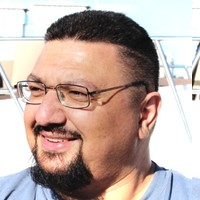
\includegraphics[width=1\linewidth]{alexei_lupan}
\end{wrapfigure}

{\Large Alexei Lupan}\\
QA analyst

\textbf{LinkedIn}:\\
\href{https://www.linkedin.com/in/testitquickly/}{testitquickly}

\textbf{Personal Website}:\\
\href{https://testitquickly.com/}{testitquickly.com}
 
\textbf{Mail}:\\
\href{mailto:astenix@testitquickly.com}{astenix@testitquickly.com} 

% \bigskip

Interested in complicated test design issues and organization of advanced trainings for new QA stuff.

Happy with baritone guitars and Robert Heinlein's books.                                                                                                                                                                                                    

% Завершение участка, в котором разруливается обрамление картинки текстом
\endgroup
